\let\negmedspace\undefined
\let\negthickspace\undefined
\documentclass[article]{IEEEtran}
\usepackage[a5paper, margin=10mm, onecolumn]{geometry}
%\usepackage{lmodern} % Ensure lmodern is loaded for pdflatex
\usepackage{tfrupee} % Include tfrupee package

\setlength{\headheight}{1cm} % Set the height of the header box
\setlength{\headsep}{0mm}     % Set the distance between the header box and the top of the text

\usepackage{gvv-book}
\usepackage{gvv}
\usepackage{cite}
\usepackage{amsmath,amssymb,amsfonts,amsthm}
\usepackage{algorithmic}
\usepackage{graphicx}
\usepackage{textcomp}
\usepackage{xcolor}
\usepackage{txfonts}
\usepackage{listings}
\usepackage{enumitem}
\usepackage{mathtools}
\usepackage{gensymb}
\usepackage{comment}
\usepackage[breaklinks=true]{hyperref}
\usepackage{tkz-euclide} 
\usepackage{listings}                                       
\def\inputGnumericTable{}                                 
\usepackage[latin1]{inputenc}                                
\usepackage{color}                                            
\usepackage{array}                                            
\usepackage{longtable}                                       
\usepackage{calc}                                             
\usepackage{multirow}                                         
\usepackage{hhline}                                           
\usepackage{ifthen}                                           
\usepackage{lscape}

\renewcommand{\thefigure}{\theenumi}
\renewcommand{\thetable}{\theenumi}
\setlength{\intextsep}{10pt} % Space between text and floats

\numberwithin{figure}{enumi}
\renewcommand{\thetable}{\theenumi}

% Marks the beginning of the document
\begin{document}
\bibliographystyle{IEEEtran}
\title{NCERT-12.8.ex.11}
\author{EE24BTECH11039 - MANDALA RANJITH}
{\let\newpage\relax\maketitle}
\noindent\textbf{Question: }  
Finding the Area Between the Parabola $y^2 = 4ax$ bounded by its latus rectum.\\\\
\solution\\
\subsection*{1. Parabola Equation in Matrix Form}
The given equation of the parabola is $y^2 = 4ax$. We can write it in matrix form as:
\begin{align}
\mathbf{x}^T \mathbf{V} \mathbf{x} + 2 \mathbf{u}^T \mathbf{x} + f = 0,
\end{align}
where:
\begin{align}
\mathbf{x} &= \begin{bmatrix} x \\ y \end{bmatrix}, \\
\mathbf{V} &= \begin{bmatrix} 0 & 0 \\ 0 & 1 \end{bmatrix}, \\
\mathbf{u} &= \begin{bmatrix} -2a \\ 0 \end{bmatrix}, \\
f &= 0.
\end{align}

Expanding this form:
\begin{align}
\begin{bmatrix} x & y \end{bmatrix}
\begin{bmatrix} 0 & 0 \\ 0 & 1 \end{bmatrix}
\begin{bmatrix} x \\ y \end{bmatrix}
+ 2 \begin{bmatrix} -2a \\ 0 \end{bmatrix}^T
\begin{bmatrix} x \\ y \end{bmatrix} + 0 &= 0.
\end{align}
This simplifies to:
\begin{align}
y^2 - 4ax &= 0,
\end{align}
which matches the given parabola equation.

The latus rectum of the parabola is the vertical line $x = a$. Substituting $x = a$ into the parabola equation:
\begin{align}
y^2 &= 4a(a), \\
y^2 &= 4a^2.
\end{align}
Taking square roots:
\begin{align}
y &= \pm 2a.
\end{align}
Thus, the limits are $-2a$ to $2a$.

\subsection*{2. Area Calculation}

\begin{align}
\text{Area} &= \int_{-2a}^{2a} \left(a - \frac{y^2}{4a}\right) \, dy.
\end{align}

\subsection*{3. Performing the Integration}

\begin{align}
\text{Area} &= \int_{-2a}^{2a} a \, dy - \int_{-2a}^{2a} \frac{y^2}{4a} \, dy.
\end{align}


\begin{align}
\int_{-2a}^{2a} a \, dy &= a \int_{-2a}^{2a} 1 \, dy = a [y]_{-2a}^{2a} = a(2a - (-2a)) = 4a^2.
\end{align}


\begin{align}
\int_{-2a}^{2a} \frac{y^2}{4a} \, dy &= \frac{1}{4a} \int_{-2a}^{2a} y^2 \, dy.
\end{align}
Now, compute $\int_{-2a}^{2a} y^2 \, dy$:
\begin{align}
\int_{-2a}^{2a} y^2 \, dy &= \left[\frac{y^3}{3}\right]_{-2a}^{2a} = \frac{(2a)^3}{3} - \frac{(-2a)^3}{3} = \frac{8a^3}{3} - \left(-\frac{8a^3}{3}\right) = \frac{16a^3}{3}.
\end{align}
Thus:
\begin{align}
\int_{-2a}^{2a} \frac{y^2}{4a} \, dy &= \frac{1}{4a} \cdot \frac{16a^3}{3} = \frac{4a^2}{3}.
\end{align}

Combining the results:\\
\begin{align}
\text{Area} &= 4a^2 - \frac{4a^2}{3} = \frac{12a^2}{3} - \frac{4a^2}{3} = \frac{8a^2}{3}.
\end{align}

\subsection*{4. Final Result}
The area between the parabola $y^2 = 4ax$ and its latus rectum $x = a$ is:
\begin{align}
\boxed{\text{Area} = \frac{8a^2}{3}}.
\end{align}



\begin{document}

\textbf{Using the trapezoidal method,}\\ 
For finding the approximate area enclosed using iterative methods, we use the Trapezoidal method. We make the area into multiple small trapeziums, and we sum up all the trapezium areas to find the total area. \\
We divide the $x$-coordinates with uniform step-size $h \to 0$, such that the discretized points are $x_0$, $x_1$, $\dots$, $x_n$ and $x_{n + 1} = x_n + h$.
\newline
Let the sum of trapezoidal areas till $x_n$ be $A_n$ and $y = y(x)$, then we write the \textbf{Difference equation},
\begin{align}
    A_n &= \frac{h}{2}(y(x_0) + y(x_1)) + \frac{h}{2}(y(x_1) + y(x_2)) + \dots + \frac{h}{2}(y(x_{n-1}) + y(x_n)) \\
    A_n &= h\left(\frac{y(x_0)}{2} + y(x_1) + y(x_2) + \dots + \frac{y(x_n)}{2}\right) \\
    A_{n+1} &= A_n + \frac{h}{2}(y(x_{n+1}) + y(x_n)) \text{, } x_{n+1} = x_n + h \\
    A_{n+1} &= A_n + \frac{h}{2}(y(x_n + h) + y(x_n)) \\
\end{align}
By the first principle of derivative,
\begin{align}
    y^{\prime}(x) &= \lim_{h\to0} \frac{y(x + h) - y(x)}{h} \\
    y(x + h) &= y(x) + h \cdot y^{\prime}(x) \text{, } h \to 0
\end{align}
Rewriting the difference equation, we get,
\begin{align}
    A_{n+1} &= A_n + \frac{h}{2}(y(x_n) + h \cdot y^{\prime}(x_n) + y(x_n)) \\
    A_{n+1} &= A_n + h(y(x_n) + \frac{h}{2} y^{\prime}(x_n)) \\
    A_{n+1} &= A_n + h \cdot y(x_n) + \frac{h^2}{2} y^{\prime}(x_n)
\end{align}\\
Divide the interval $[0, a]$ into $n$ subintervals of width $h = \frac{a-0}{n} = \frac{a}{n}$. Let $x_0 = 0$, $x_1 = h$, $x_2 = 2h$, $\dots$, $x_n = a$.

The trapezoidal method for numerical integration is given by:
\begin{align}
  A \approx \frac{h}{2} \left[ f(x_0) + 2 \sum_{i=1}^{n-1} f(x_i) + f(x_n) \right]  
\end{align}

where $f(x) = \sqrt{4ax}$.

Since we need to account for both the positive and negative branches of the parabola, we use \( f(x) = \sqrt{4ax} \) for the upper part of the parabola and \( f(x) = -\sqrt{4ax} \) for the lower part. The total area is the sum of the areas above and below the x-axis, so we take the absolute value of \( y \). Hence, we use \( |f(x)| = \sqrt{4ax} \) for both branches.

Substitute $f(x)$ into the formula:
\begin{align}
    A \approx \frac{h}{2} \left[ \left( \sqrt{4a \cdot x_0} \right) + 2 \sum_{i=1}^{n-1} \left( \sqrt{4a \cdot x_i} \right) + \left( \sqrt{4a \cdot x_n} \right) \right].
\end{align}
\textbf{Numerical Approach}\\

To approximate the area of the region using the trapezoidal method, we adopt the following numerical approach. This method involves iteratively calculating the area using discrete steps:

\textbf{Initialization:}
\begin{itemize}
    \item Start with initial values $x_0 = 0$ and $A_0 = 0$.
    \item Set the step size $h = \frac{a}{n}$, where $n$ is the number of subintervals.
\end{itemize}

\textbf{Iterative formulae:}\\
\begin{itemize}
    \item For each iteration $i$ from 1 to $n$, perform the following steps:
    \begin{itemize}
        \item[1.] Compute $y_i = \sqrt{4a \cdot x_i}$.
        \item[2.] Update the area sum using:
        \begin{align}
        A_i &= A_{i-1} + \frac{1}{2} h (y_i + y_{i-1})
        \end{align}
        \item[3.] Update $x_i$ for the next iteration using:
        \begin{align}
        x_i &= x_{i-1} + h
        \end{align}
    \end{itemize}
\end{itemize}

\textbf{Final Area Calculation:}\\
\begin{itemize}
    \item After completing all iterations, the final approximate area $A_n$ is:
    \begin{align}
    A &= A_n
    \end{align}
\end{itemize}

\textbf{Initial Conditions:}
\begin{itemize}
    \item $x_0 = 0$
    \item $A_0 = 0$
    \item $h = \frac{a}{n}$ (depending on the chosen number of subintervals $n$)
    \item Here we assume $n = 30$.
\end{itemize}

This approach ensures an accurate approximation of the area by iteratively applying the trapezoidal rule, leveraging the discretized nature of the integral.\\
$ \implies$ The theoretical value of Area is $\frac{a^2}{2}$\\
$ \implies$ The computational value of Area is obtained using the trapezoidal method.\\
Therefore, we can claim that the trapezoidal rule/method for finding area works well.

\begin{figure}[h!]
	\centering
	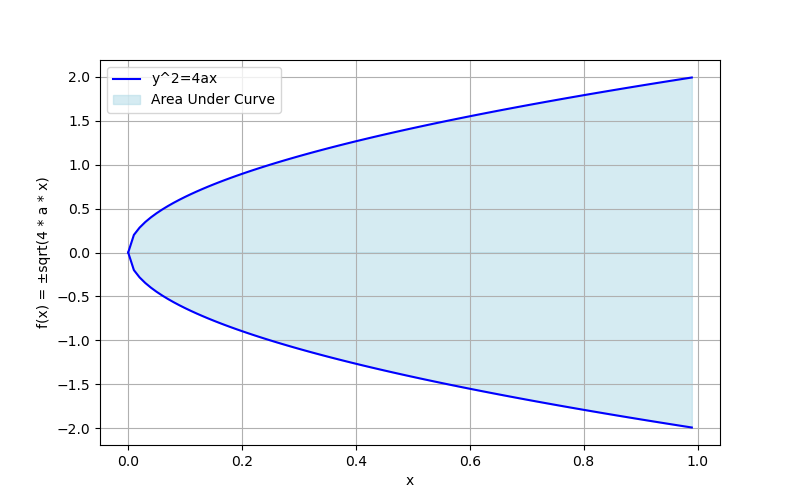
\includegraphics[width=\columnwidth]{figures/Figure_1.png}
	\caption{Area function graph.}
	\label{stemplot}
\end{figure}

\end{document}

\end{document}

